\documentclass[11pt,aspectratio=43,xcolor=table]{beamer}

%------------------------------------------------
% Theme
%------------------------------------------------
\usetheme{Madrid}
\usefonttheme{serif}
\usepackage{tikz}
\usepackage{tabularx}
\usepackage{booktabs}
\usepackage{array}

% Define custom column types used in your table
\newcolumntype{L}[1]{>{\raggedright\arraybackslash}p{#1}}
\newcolumntype{Z}{>{\raggedright\arraybackslash}X}

% Define \strong if you don't already have it
\providecommand{\strong}[1]{\textbf{#1}}
\usetikzlibrary{shapes.geometric, arrows.meta, positioning, fit, backgrounds, calc}

% Set bibliography style to numbered text citations [1], [2], ...
\setbeamertemplate{bibliography item}[text]

%------------------------------------------------
% Colors
%------------------------------------------------
\definecolor{AegisBlue}{RGB}{52,50,181}
\setbeamercolor{structure}{fg=AegisBlue}
\setbeamercolor{frametitle}{bg=AegisBlue,fg=white}
\setbeamercolor{title}{bg=AegisBlue,fg=white}
\date{September 17, 2026}

%================================================
\begin{document}

%------------------------------------------------
% Slide 1 - Title Slide
%------------------------------------------------
\begin{frame}
\centering

%------------------------------------------------
% Blue Title Box
%------------------------------------------------
\begin{beamercolorbox}[
    wd=1\textwidth,
    rounded=true,
    shadow=true,
    sep=9pt,
    center
]{title}

\Large\bfseries
Analyzing Bias Propagation in Recommender Feedback Loops Using Embeddings

\end{beamercolorbox}

\vspace{0.5cm}

\small
\begin{tabular}{l l}
Anirudh S Nair & TVE23CS037 \\
Navya M J & TVE23CS100 \\
Niharika S & TVE23CS105 \\
Shravan Nander Pandala & TVE23CS131 \\
\end{tabular}

\vspace{0.4cm}

\normalsize \textbf{September 17, 2026}

\vspace{0.3cm}
\normalsize
\textbf{Project Guide}

\vspace{0.1cm}

\small
Dr.\ Ajeesh Ramanujan\\
Associate Professor\\
Department of Computer Science and Engineering\\
College of Engineering Trivandrum

\end{frame}

%------------------------------------------------
% Slide 2 - Contents
%------------------------------------------------
\begin{frame}{Contents}
\tableofcontents
\end{frame}

\begin{frame}{Feedback Loop Bias Example}
\scriptsize

\textbf{Spotify}

\bigskip

\centering
Listen to \textit{Popular Artist}
$\rightarrow$
Recommend Similar Popular Songs
$\rightarrow$
User Streams Recommended Songs
$\rightarrow$
Model Learns Strong Preference for Popular Artists
$\rightarrow$
Recommend More Popular Music

\bigskip

\raggedright
\textbf{Feedback Loop:} Recommendations shape user listening behavior, which becomes new training data. Repeated cycles reinforce popularity bias and reduce exposure to less-popular artists and diverse genres.

\end{frame}

%================================================
\section{Introduction}
%================================================

%------------------------------------------------
% Slide 3 - Introduction & Domain of Interest
%------------------------------------------------
\begin{frame}{Introduction}
\small

\begin{itemize}
    \item Recommender systems represent users and items as \textbf{latent vector embeddings}.
    \item Recommendations influence future user interactions, creating a \textbf{closed feedback loop}.
    \item Repeated retraining can amplify \textbf{popularity bias} and cause changes in embedding geometry.
\end{itemize}

\vspace{0.2cm}

\textbf{Domain of Interest}

\begin{itemize}
    \item Recommender Systems
    \item Vector Embeddings
    \item Closed Feedback Loops
    \item Embedding Geometry
\end{itemize}

\end{frame}

%================================================
\section{Problem Context}
%================================================

%------------------------------------------------
% Slide 4 - Problem Context
%------------------------------------------------
\begin{frame}{Problem Context}

\begin{itemize}
    \item \textbf{Systemic Observational Bias}: Historical training logs contain inherent observational bias and do not accurately reflect true user tastes.
    \item \textbf{Algorithmic Reinforcement}: Standard collaborative models disproportionately favor popular items while neglecting the majority of catalog items.
    \item \textbf{Dynamic Feedback Amplification}: Rather than staying static, feedback loop bias is self-reinforcing, growing progressively stronger with each subsequent retraining generation.
    \item \textbf{Degradation of Personalization}: Niche users are increasingly deprived of recommendations that cater to their genuine, diverse interests.
\end{itemize}

\end{frame}

%================================================
\section{Literature Review}
%================================================

% ------------- SLIDE 1: Zoralioglu & Yalcin (2026) -------------
\begin{frame}{Literature Survey}
\small
\textbf{Paper:} \emph{Dynamic Feedback Loops in Recommender Systems} \\
\textbf{Authors:} Zoralioglu \& Yalcin (2026)

\vspace{0.15cm}
\begin{block}{Significance to Our Project}
\begin{itemize}
  \item Provides baseline conceptual framework for multi-generation ($T=10$) closed-loop simulations.
  \item Demonstrates progressive exposure degradation and calibration loss across retraining iterations.
\end{itemize}
\end{block}

\vspace{0.05cm}
\begin{block}{Research Gap Identified}
\begin{itemize}
  \item Evaluates system degradation strictly via surface-level recommendation lists.
  \item Lacks vector-space geometric tracking (fails to measure embedding drift velocity, coordinate variance collapse, or spatial deformation).
\end{itemize}
\end{block}
\end{frame}

% ------------- SLIDE 2: Mansoury et al. (2020) -------------
\begin{frame}{Literature Survey}
\small
\textbf{Paper:} \emph{Feedback Loop and Bias Amplification in Recommender Systems} \\
\textbf{Authors:} Mansoury et al. (2020)

\vspace{0.15cm}
\begin{block}{Significance to Our Project}
\begin{itemize}
  \item Pioneers empirical closed-loop offline simulation across standard CF algorithms (\texttt{UserKNN}, \texttt{BPR}, \texttt{MostPopular}).
  \item Proves feedback loops amplify popularity bias (Matthew Effect) and systematically reduce catalog diversity.
\end{itemize}
\end{block}

\vspace{0.05cm}
\begin{block}{Research Gap Identified}
\begin{itemize}
  \item Relies on static, non-adaptive user acceptance rules without position decay or popularity conformity dynamics.
  \item Fails to analyze internal representation dynamics (cannot differentiate pointwise origin collapse from pairwise periphery dispersion).
\end{itemize}
\end{block}
\end{frame}

% ------------- SLIDE 3: Salah et al. (2020) [Cornac] -------------
\begin{frame}{Literature Survey}
\small
\textbf{Paper:} \emph{Cornac: A Comparative Multimodal Framework for Recommendation} \\
\textbf{Authors:} Salah et al. (2020)

\vspace{0.15cm}
\begin{block}{Significance to Our Project}
\begin{itemize}
  \item Core recommendation execution engine utilized in our research framework (Phase 2 benchmarking \& Subsystem 2 adapters).
  \item Enables unified, reproducible training of matrix factorization (\texttt{MF}, \texttt{PMF}, \texttt{BPR}) and memory-based models.
\end{itemize}
\end{block}

\vspace{0.05cm}
\begin{block}{Research Gap Identified}
\begin{itemize}
  \item Architected exclusively for static, single-pass offline model evaluation.
  \item Lacks native support for multi-generation feedback loop execution, dynamic data buffer accumulation, and geometric coordinate drift tracking.
\end{itemize}
\end{block}
\end{frame}

% ------------- SLIDE 4: Liu et al. (2026) [CDSRec] -------------
\begin{frame}{Literature Survey}
\small
\textbf{Paper:} \emph{Causal Disentanglement for Tackling Popularity Bias (CDSRec)} \\
\textbf{Authors:} Liu et al. (2026)

\vspace{0.15cm}
\begin{block}{Significance to Our Project}
\begin{itemize}
  \item Establishes a Structural Causal Model (SCM) to separate intrinsic item quality from trend exposure bias.
  \item Serves as the state-of-the-art causal debiasing reference benchmark for Phase 4 mitigation strategies.
\end{itemize}
\end{block}

\vspace{0.05cm}
\begin{block}{Research Gap Identified}
\begin{itemize}
  \item High architectural complexity (Markov chains, DAGs, VAEs) tailored for single-pass sequential interaction logs.
  \item Does not measure geometric embedding space contraction or latent coordinate drift under continuous closed-loop retraining.
\end{itemize}
\end{block}
\end{frame}

% ------------- SLIDE 5: Chaney et al. (2018) -------------
\begin{frame}{Literature Survey}
\small
\textbf{Paper:} \emph{How Algorithmic Confounding Increases Homogeneity and Decreases Utility} \\
\textbf{Authors:} Chaney et al. (2018)

\vspace{0.15cm}
\begin{block}{Significance to Our Project}
\begin{itemize}
  \item Early multi-generation agent simulation showing recommendation loops cause user preference homogenization and utility decay.
  \item Demonstrates how user interaction choices become confounded by prior algorithmic exposure.
\end{itemize}
\end{block}

\vspace{0.05cm}
\begin{block}{Research Gap Identified}
\begin{itemize}
  \item Relies on idealized synthetic user utility functions rather than empirical interaction datasets (e.g., MovieLens 1M).
  \item Ignores latent representation mechanics, vector coordinate space dynamics, and model-specific geometric failure modes.
\end{itemize}
\end{block}
\end{frame}

% ------------- SLIDE 6: Summary of Other Literature -------------
\begin{frame}{Literature Survey}
\small
\textbf{Baseline \& Survey Literature Summary}

\vspace{0.1cm}
\scriptsize
\setlength{\tabcolsep}{1.5pt}
\renewcommand{\arraystretch}{1.1}
\begin{tabularx}{\textwidth}{L{2.0cm} Z Z Z}
\toprule
\strong{Paper} & \strong{Focus / Methodology} & \strong{Key Findings} & \strong{Limitations / Gaps} \\
\midrule
Chen et al. (2023) & Debiasing survey (IPS, Causal, RL). & Identifies feedback loops as primary bias driver. & Qualitative survey; lacks empirical vector dynamics. \\
\midrule
Ma et al. (2019) & MacridVAE via Variational Autoencoders. & Separates macro/micro intentions in latent space. & Learned dimensions lack interpretability without attributes. \\
\midrule
Kang \& McAuley (2018) & SASRec (Self-Attention Sequential). & Captures long/short-term sequential preferences. & Cannot scale efficiently; ignores feedback loop vector drift. \\
\midrule
Hidasi et al. (2016) & GRU4Rec (Gated Recurrent Units). & Models session click transitions. & Relies strictly on item IDs; ignores content features. \\
\midrule
Rendle et al. (2009) & BPR (Pairwise SGD ranking). & Optimizes relative item ordering over implicit logs. & Static model; vulnerable to periphery dispersion under loops. \\
\bottomrule
\end{tabularx}
\end{frame}

%================================================
\section{Research Gap}
%================================================

%------------------------------------------------
% Slide 15 - Research Gap
%------------------------------------------------
\begin{frame}{Critical Research Gaps}
  \begin{itemize}
    \setlength{\itemsep}{14pt}
    \item \textbf{Research Gap 1: Static vs. Dynamic Bias}
    \begin{itemize}
      \setlength{\itemsep}{5pt}
      \item Existing mitigation strategies treat bias predominantly as a static problem.
      \item Current models fail to account for how sequential feedback loops compound and amplify bias across iterative retraining cycles.
    \end{itemize}

    \item \textbf{Research Gap 2: Structural Vector Analysis}
    \begin{itemize}
      \setlength{\itemsep}{5pt}
      \item Prior literature emphasizes surface recommendation metrics over internal latent representations.
      \item Standard benchmarks do not quantify the geometric drift, topological deformation, or contraction of vector embeddings during retraining loops.
    \end{itemize}
  \end{itemize}
\end{frame}

\begin{frame}{Bridging the Research Gap}
  \begin{itemize}
    \setlength{\itemsep}{12pt}
    \item \textbf{Mathematical Drift Metrics}
    \begin{itemize}
      \setlength{\itemsep}{3pt}
      \item Formulate quantitative metrics to track embedding displacement vectors, trajectory divergence, and contraction velocity across retraining iterations.
    \end{itemize}

    \item \textbf{Latent Space Preservation}
    \begin{itemize}
      \setlength{\itemsep}{3pt}
      \item Systematically design and evaluate algorithmic safeguards, regularization constraints, and update bounds that prevent latent space collapse.
    \end{itemize}

    \item \textbf{Catalog Coverage \& Fairness}
    \begin{itemize}
      \setlength{\itemsep}{3pt}
      \item Preserve long-term item catalog exposure equity and safeguard recommendation quality for user groups with niche preferences.
    \end{itemize}
  \end{itemize}
\end{frame}

%================================================
\section{Problem Statement}
%================================================

%------------------------------------------------
% Slide 16 - Problem Statement
%------------------------------------------------
\begin{frame}{Problem Statement}

\vfill

\begin{block}{Problem}
\centering
Analyze and mitigate dynamic bias propagation in closed-loop recommender systems by tracking and stabilizing latent embedding drift and spatial contraction across retraining cycles to prevent catalog coverage collapse and protect niche user preferences.
\end{block}

\vfill

\end{frame}

%================================================
\section{Project Objectives}
%================================================

%------------------------------------------------
% Slide 17 - Project Objectives
%------------------------------------------------
\begin{frame}{Project Objectives}

\begin{block}{Primary Objective}
Analyze and mitigate dynamic bias propagation in closed-loop
recommender systems by tracking geometric changes in vector
embedding space.
\end{block}

\vspace{0.2cm}

\textbf{Specific Objectives}
\begin{itemize}
    \item Build Simulation Framework: Construct a closed-loop
simulation environment to model multi-generation
recommendation cycles.
    \item Quantify Vector Contraction: Calculate the velocity of
embedding space contraction to measure diversity loss and
popularity concentration.
    \item Evaluate Mitigation Methods: Test alternative
recommendation algorithms and bias mitigation techniques to
stabilize vector trajectories.
\end{itemize}

\end{frame}

%================================================
\section{Proposed Solution Methodology}
%================================================

%------------------------------------------------
% Slide 18 - Overall Methodology
%------------------------------------------------
\begin{frame}{Proposed Solution Methodology -- Overview}
  \begin{itemize}
      \item The system consists of five sequential stages: \textbf{baseline anchoring}, \textbf{model recommendation}, \textbf{stochastic click simulation}, \textbf{data ingestion (the feedback loop)}, and \textbf{diagnostic auditing}.
      \vspace{0.5cm}
      \item Two core pipelines define the system: a \textbf{closed-loop simulation pipeline} (modeling user clicks based on exposure, relevance, and conformity) and a \textbf{4-tier diagnostic pipeline} (measuring popularity bias propagation and latent space degradation).
  \end{itemize}
\end{frame}

% Slide 19
\begin{frame}{System Setup \& Baseline Initialization}
    \begin{itemize}
        \item \textbf{Data Ingestion:} Ingest the MovieLens-1M dataset and binarize the historical user-item interactions.
        \item \textbf{Baseline Training:} Train the suite of recommender models (Matrix Factorization, BPR, PMF, UserKNN) on this initial dataset.
        \item \textbf{Preference Freezing:} Extract and freeze a ``Ground-Truth Anchor'' from these baseline models. This serves as a permanent, uncorrupted record of the users' original preferences before the simulation begins.
    \end{itemize}
\end{frame}

% Slide 20
\begin{frame}{Simulating User Interactions}
    \begin{itemize}
        \item \textbf{Recommendation Generation:} Generate Top-$K$ candidate lists for all users from freshly trained models.
        \item \textbf{Exposure Discount:} Scale click likelihood via a position-based rank decay.
        \item \textbf{Relevance Matching:} Score true intrinsic utility against the Frozen Ground-Truth Anchor.
        \item \textbf{Social Conformity:} Inject a bandwagon boost for platform-wide popular items.
        \item \textbf{Click Sampling:} Synthesize exposure, relevance, and conformity into final clicks under session fatigue caps.
    \end{itemize}
\end{frame}

% Slide 21
\begin{frame}{Closing the Loop \& Measuring Bias}
    \begin{itemize}
        \item \textbf{Feedback Loop Ingestion:} Append simulated clicks into the interaction matrix as new observations.
        \item \textbf{Iterative Retraining:} Retrain models on augmented logs to simulate self-reinforcing bias cycles.
        \item \textbf{Macro-Distribution Analysis:} Track catalog concentration via Exposure Gini and Catalog Coverage.
        \item \textbf{Subgroup Taste Distortion:} Measure drift between niche user recommendations and baseline profiles.
        \item \textbf{Latent Degradation:} Track representation collapse via Effective Spectral Rank on aligned embeddings.
    \end{itemize}
\end{frame}

%================================================
\section{System Architecture}
%================================================

%------------------------------------------------
% Slide 22 - System Architecture
%------------------------------------------------
\begin{frame}{System Architecture}

\begin{figure}
    \centering
    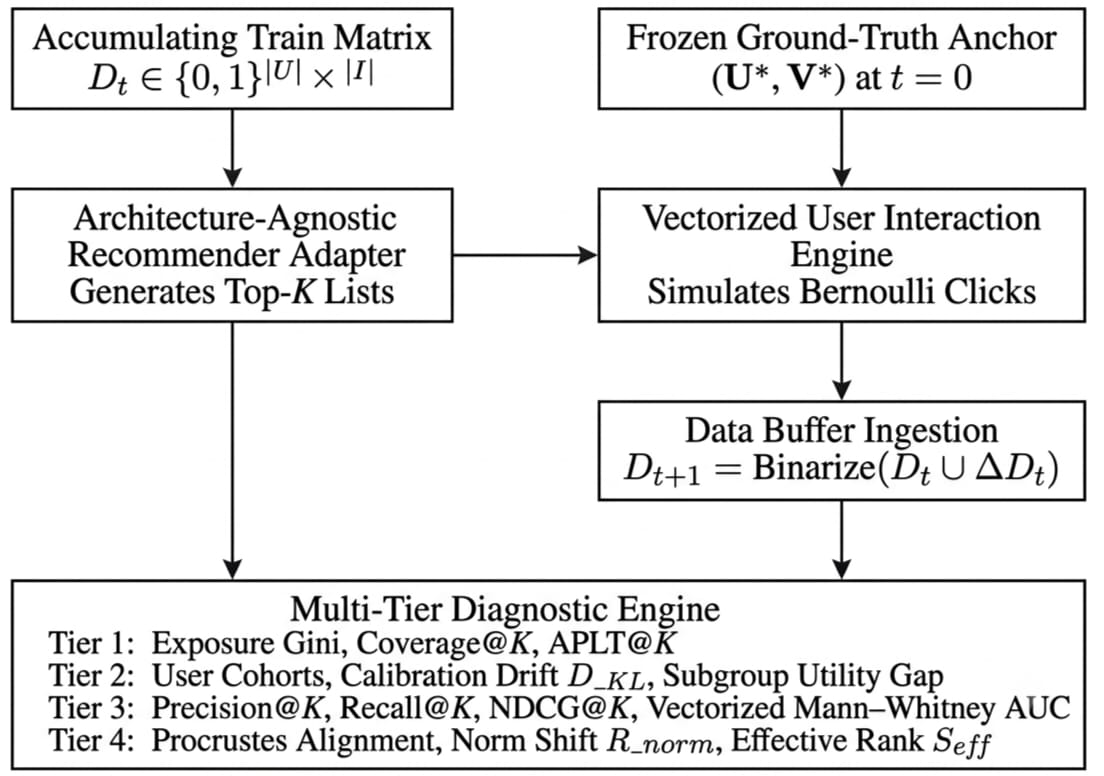
\includegraphics[height=0.78\textheight,keepaspectratio]{phase_4_architecture.jpeg}
    \caption{Proposed System Architecture}
\end{figure}

\end{frame}

%------------------------------------------------
% Slide 23 - Flow Diagram
%------------------------------------------------
\begin{frame}{Flow Diagram of Proposed System}

\begin{figure}[htpb]
\centering
\resizebox{!}{0.7\textheight}{%
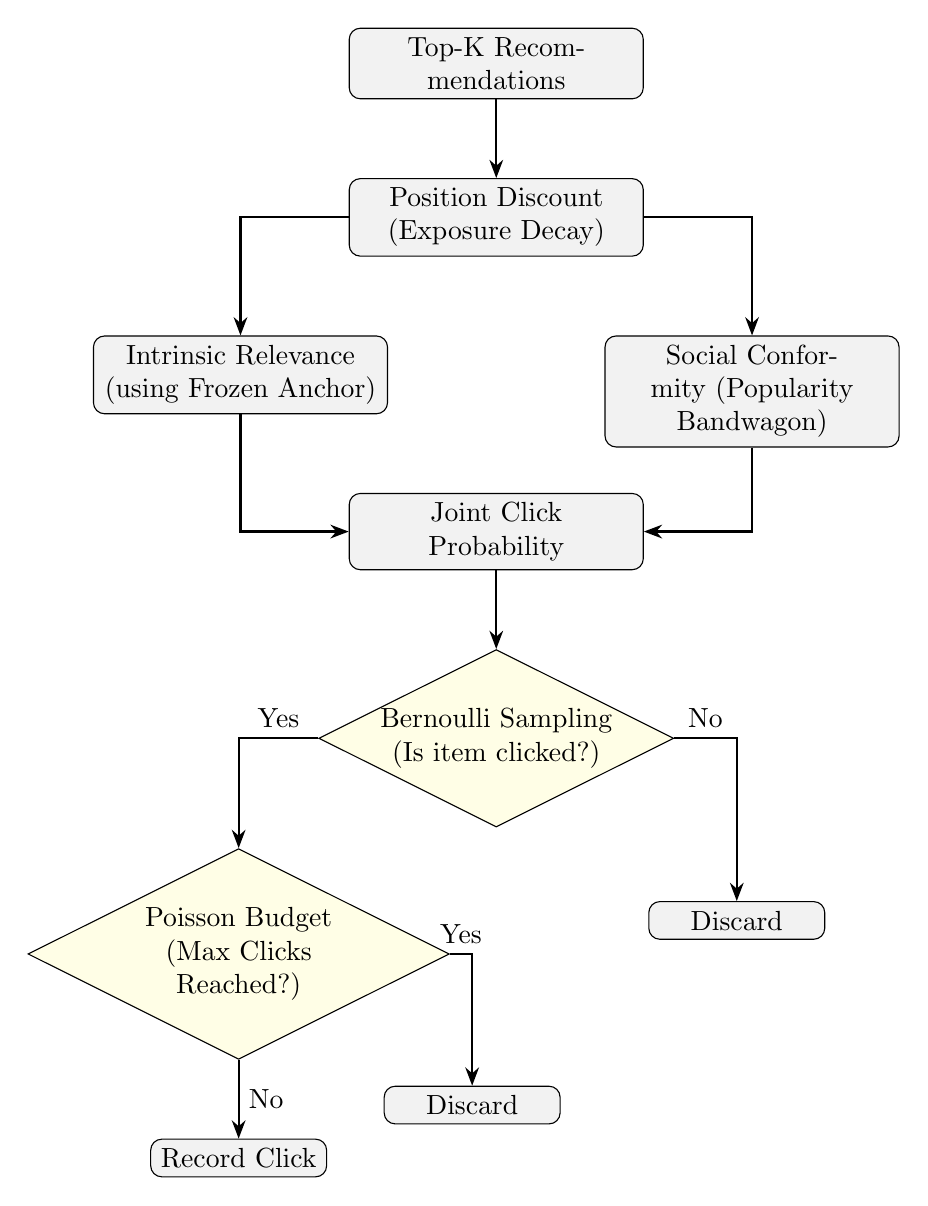
\begin{tikzpicture}[
    node distance=1cm and 0.5cm,
    box/.style={draw, rectangle, rounded corners, align=center, text width=3.5cm, fill=gray!10},
    decision/.style={draw, diamond, aspect=2, align=center, text width=3cm, fill=yellow!10, inner sep=0pt},
    arrow/.style={-{Stealth}, thick}
]

% Nodes
\node[box] (start) {Top-K Recommendations};
\node[box, below=of start] (exp) {Position Discount (Exposure Decay)};

\node[box, below left=1cm and -0.5cm of exp] (rel) {Intrinsic Relevance (using Frozen Anchor)};
\node[box, below right=1cm and -0.5cm of exp] (conf) {Social Conformity (Popularity Bandwagon)};

\node[box, below=3cm of exp] (joint) {Joint Click Probability};

\node[decision, below=of joint] (sample) {Bernoulli Sampling (Is item clicked?)};

\node[decision, below left=1.5cm and 0.8cm of sample] (budget) {Poisson Budget (Max Clicks Reached?)};
\node[box, below right=1.5cm and 0.8cm of sample, text width=2cm] (discard1) {Discard};

\node[box, below=1cm of budget, text width=2cm] (record) {Record Click};
\node[box, below right=1cm and 0.5cm of budget, text width=2cm] (discard2) {Discard};

% Arrows
\draw[arrow] (start) -- (exp);
\draw[arrow] (exp) -| (rel);
\draw[arrow] (exp) -| (conf);
\draw[arrow] (rel) |- (joint);
\draw[arrow] (conf) |- (joint);
\draw[arrow] (joint) -- (sample);

\draw[arrow] (sample.west) -| node[above, near start] {Yes} (budget.north);
\draw[arrow] (sample.east) -| node[above, near start] {No} (discard1.north);

\draw[arrow] (budget.south) -- node[right] {No} (record.north);
\draw[arrow] (budget.east) -| node[above, near start] {Yes} (discard2.north);

\end{tikzpicture}%
}

\caption{Vectorized User Interaction Flow}
\end{figure}

\end{frame}

%------------------------------------------------
% Slide 24 - Block Diagram
%------------------------------------------------
\begin{frame}{Block Diagram of Proposed System}
\begin{figure}[htpb]
\centering
\resizebox{0.9\textwidth}{!}{%
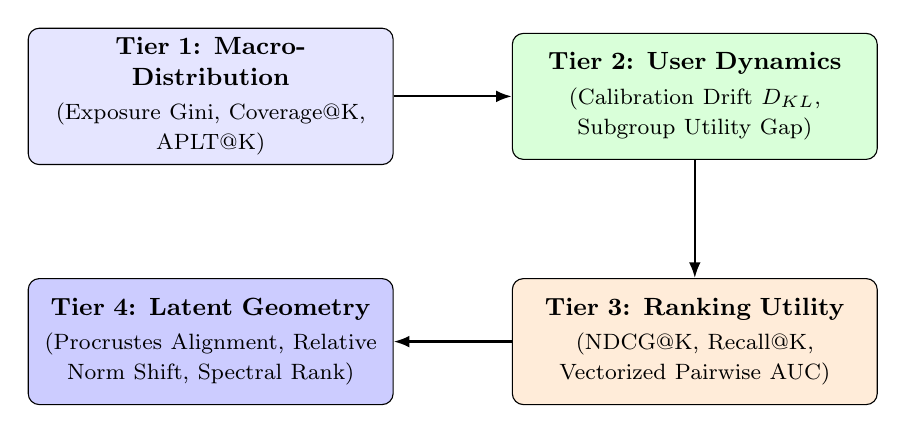
\begin{tikzpicture}[
    block/.style={draw, rounded corners, minimum height=1.6cm, minimum width=3.6cm, text width=4.4cm, align=center, font=\small},
    arr/.style={-{Latex[length=2mm]}, thick}
  ]
  
  % Tier 1 (Top Left)
  \node[block, fill=blue!10] (t1) {\textbf{Tier 1: Macro-Distribution}\\[1mm]\footnotesize (Exposure Gini, Coverage@K,\\APLT@K)};
  
  % Tier 2 (Top Right)
  \node[block, right=1.5cm of t1, fill=green!15] (t2) {\textbf{Tier 2: User Dynamics}\\[1mm]\footnotesize (Calibration Drift $D_{KL}$,\\Subgroup Utility Gap)};
  
  % Tier 3 (Bottom Right)
  \node[block, below=1.5cm of t2, fill=orange!15] (t3) {\textbf{Tier 3: Ranking Utility}\\[1mm]\footnotesize (NDCG@K, Recall@K,\\Vectorized Pairwise AUC)};
  
  % Tier 4 (Bottom Left)
  \node[block, left=1.5cm of t3, fill=blue!20] (t4) {\textbf{Tier 4: Latent Geometry}\\[1mm]\footnotesize (Procrustes Alignment, Relative\\Norm Shift, Spectral Rank)};

  % Arrows connecting the tiers in a U-shape sequence (1 -> 2 -> 3 -> 4)
  \draw[arr] (t1) -- (t2);
  \draw[arr] (t2) -- (t3);
  \draw[arr] (t3) -- (t4);
  
\end{tikzpicture}}
\caption{Multi-Tier Diagnostic Auditing Progression}
\end{figure}

\end{frame}

%================================================
\section{Project Planning}
%================================================

%------------------------------------------------
% Slide 25 - Project Planning
%------------------------------------------------
\begin{frame}[t]{Project Planning}
\begin{block}{Project Schedule}
\resizebox{\linewidth}{!}{%
\renewcommand{\arraystretch}{1.25}
\begin{tabular}{llccccccc}

\textcolor{black}{\textbf{Phase}} &
\textcolor{black}{\textbf{Activity}} &
\textcolor{black}{\textbf{Sep}} &
\textcolor{black}{\textbf{Oct}} &
\textcolor{black}{\textbf{Nov}} &
\textcolor{black}{\textbf{Dec}} &
\textcolor{black}{\textbf{Jan}} &
\textcolor{black}{\textbf{Feb}} &
\textcolor{black}{\textbf{Mar}} \\ \hline

\textbf{Planning} & Literature Survey
    & \cellcolor{AegisBlue!35} & & & & & & \\
& System Design
    & \cellcolor{AegisBlue!35} & \cellcolor{AegisBlue!35} & & & & & \\ \hline

\textbf{Development} & Data Pipeline \& Preprocessing
    & & \cellcolor{AegisBlue!35} & \cellcolor{AegisBlue!35} & & & & \\
& Recommender Adapters (Cornac)
    & & & \cellcolor{AegisBlue!35} & \cellcolor{AegisBlue!35} & & & \\
& User Interaction Engine (Feedback Loop)
    & & & & \cellcolor{AegisBlue!35} & \cellcolor{AegisBlue!35} & & \\
& Diagnostic Auditing Engine (Metrics)
    & & & & & \cellcolor{AegisBlue!35} & \cellcolor{AegisBlue!35} & \\ \hline

\textbf{Testing} & Full-Loop Integration \& Testing
    & & & & & & \cellcolor{AegisBlue!35} & \cellcolor{AegisBlue!35} \\
& Performance Evaluation
    & & & & & & \cellcolor{AegisBlue!35} & \cellcolor{AegisBlue!35} \\

\end{tabular}%
}
\end{block}

\end{frame}

%================================================
\section{Conclusion}
%================================================

%------------------------------------------------
% Slide 26 - Conclusion
%------------------------------------------------
\begin{frame}{Conclusion}
    \begin{itemize}
        \item Proposed a robust closed-loop simulation framework to model popularity bias propagation in recommender systems.
        \item Integrates architecture-agnostic collaborative filtering models with a stochastic, vectorized user interaction engine.
        \item Enables comprehensive, multi-tier diagnostic auditing of macro-inequality, user taste distortion, and latent space degradation.
        \item Establishes a scalable baseline for evaluating bias mitigation algorithms and long-term representation fairness in continuous feedback cycles.
    \end{itemize}
\end{frame}

%================================================
\section{References}
%================================================

%------------------------------------------------
% Slide 27 - References
%------------------------------------------------
\begin{frame}[allowframebreaks]{References}
  \footnotesize
  \begin{thebibliography}{99}
    \bibitem{zoralioglu} H. Zoralioglu, C. Yalcin, ``Dynamic Feedback Loops in Recommender Systems,'' 2026.
    \bibitem{liu} Y. Liu et al., ``Causal Disentanglement for Tackling Popularity Bias,'' 2026.
    \bibitem{chen} J. Chen, H. Dong, X. Wang, F. Feng, M. Wang, T.-S. Chua, ``Bias and Debias in Recommender System: A Survey and Future Directions,'' \emph{ACM Trans. Inf. Syst.}, vol. 41, no. 3, pp. 1--39, 2023.
    \bibitem{mansoury} M. Mansoury, H. Abdollahpouri, M. Pechenizkiy, B. Mobasher, R. Burke, ``Feedback Loop and Bias Amplification in Recommender Systems,'' in \emph{Proc. 29th ACM Int. Conf. Inf. Knowl. Manag. (CIKM)}, 2020, pp. 2145--2148.
    \bibitem{salah} A. Salah, Q. T. Truong, H. W. Lauw, ``Cornac: A Comparative Framework for Multimodal Recommender Systems,'' \emph{J. Mach. Learn. Res.}, vol. 21, no. 95, pp. 1--5, 2020.
    \bibitem{ma} J. Ma, C. Zhou, P. Cui, H. Yang, W. Zhu, ``Learning Disentangled Representations for Recommendation,'' in \emph{Proc. 33rd Conf. Neural Inf. Process. Syst. (NeurIPS)}, 2019, pp. 5711--5722.
    \bibitem{chaney} A. J. B. Chaney, B. M. Stewart, B. E. Engelhardt, ``How Algorithmic Confounding Increases Homogeneity and Decreases Utility,'' in \emph{Proc. 12th ACM Conf. Recommender Syst. (RecSys)}, 2018, pp. 224--232.
    \bibitem{kang} W.-C. Kang, J. McAuley, ``Self-Attentive Sequential Recommendation,'' in \emph{Proc. IEEE Int. Conf. Data Min. (ICDM)}, 2018, pp. 197--206.
    \bibitem{hidasi} B. Hidasi, A. Karatzoglou, L. Baltrunas, D. Tikk, ``Session-based Recommendations with Recurrent Neural Networks,'' in \emph{Proc. 4th Int. Conf. Learn. Represent. (ICLR)}, 2016.
    \bibitem{rendle} S. Rendle, C. Freudenthaler, Z. Gantner, L. Schmidt-Thieme, ``BPR: Bayesian Personalized Ranking from Implicit Feedback,'' in \emph{Proc. 25th Conf. Uncertainty Artif. Intell. (UAI)}, 2009, pp. 452--461.
  \end{thebibliography}
\end{frame}

% =========================================================
\begin{frame}
  \centering
  \Huge Thank You!
\end{frame}

\end{document}